La era tecnológica ha avanzado en los últimos años a pasos agigantados, y las
demandas del sector han crecido junto a ella. No hace más de 200 años se ``descubría''
la electricidad; hace 90 años nacía la primera computadora básica capaz de realizar
operaciones aritméticas; hace 70 años nacía el transistor que sustituyó las
válvulas de vacío (figura \ref{fig:transistor}); y desde entonces, el crecimiento
ha sido exponencial \cite{HistoryTechnologyTimeline}.

\begin{figure}[H]
    \centering
    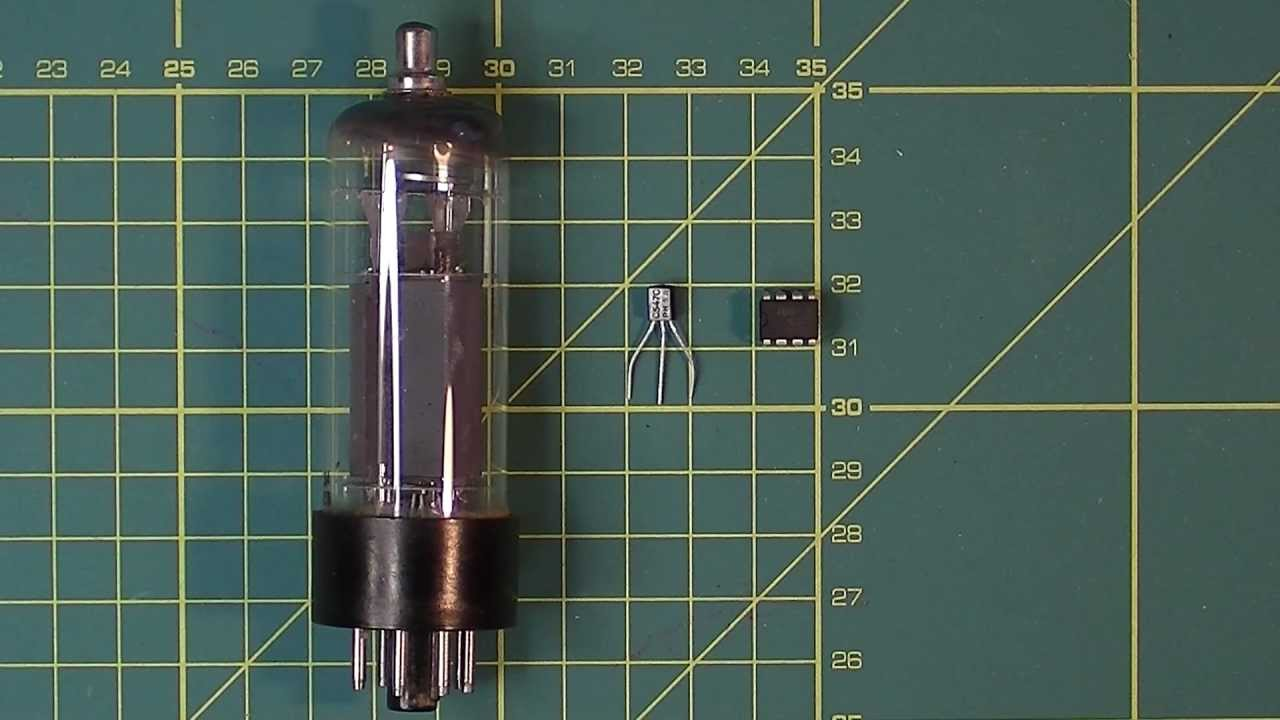
\includegraphics[width=.7\linewidth]{pictures/transistor-vs-valve.jpg}
    \caption{Comparativa de una válvula de vacío (izquierda) frente a un transistor (centro) y un circuito integrado (derecha).}
    \label{fig:transistor}
\end{figure}

Otro de los ejemplos de tecnologías que han crecido exponencialmente son los dispositivos
de almacenamiento, donde no hacía más de 20 años las capacidades máximas se estimaban
en torno a los MB (megabytes) y ahora se hablan de EB (exabytes) \cite{EvolutionDataStorage}.
Esta evolución es muy representativa también a nivel económico, ya que el coste del
almacenamiento ha ido bajando a medida pasaba el tiempo, así como el espacio físico
que ocupan los dispositivos (figura \ref{fig:disk-evolution}):

\begin{figure}[H]
    \centering
    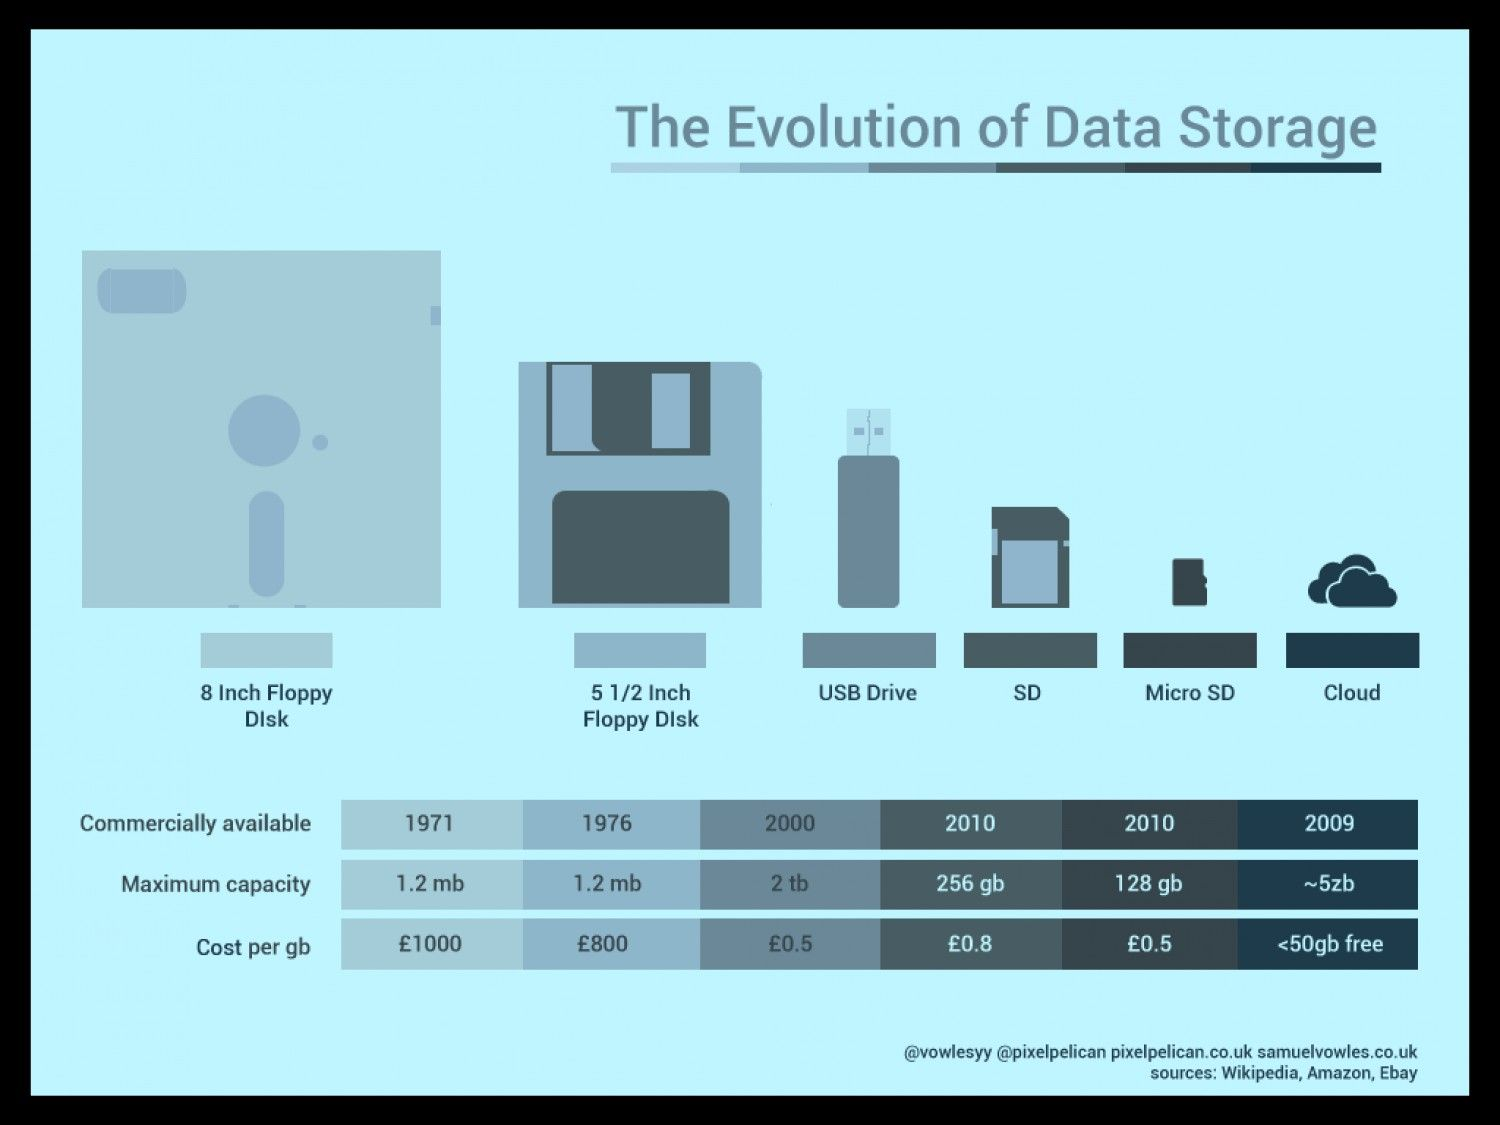
\includegraphics[width=.65\linewidth]{pictures/disk-evo.jpg}
    \caption{Evolución del espacio de almacenamiento en términos económicos y cuantitativos \cite{wecomputingtechStorageDevicesLondon}.}
    \label{fig:disk-evolution}
\end{figure}

Finalmente, el gran salto tecnológico se ha producido con la aparición de Internet y
las comunicaciones ya no eran únicamente personales sino entre dispositivos. En relación
con el punto anterior, la aparición de Internet ha permitido descentralizar el espacio
donde ya el usuario no guarda su información en su equipo personal sino en un clúster
de servidores distribuidos a nivel mundial al cual accede, de forma simultánea,
desde Internet y desde cualquier dispositivo. Así, lo que comenzó como una red de
conexión de unos pocos usuarios ha acabado convirtiéndose en la red global que
todos usamos y que conecta más de 4 billones de dispositivos (figura \ref{fig:internet-evo}).

\begin{figure}[H]
    \centering
    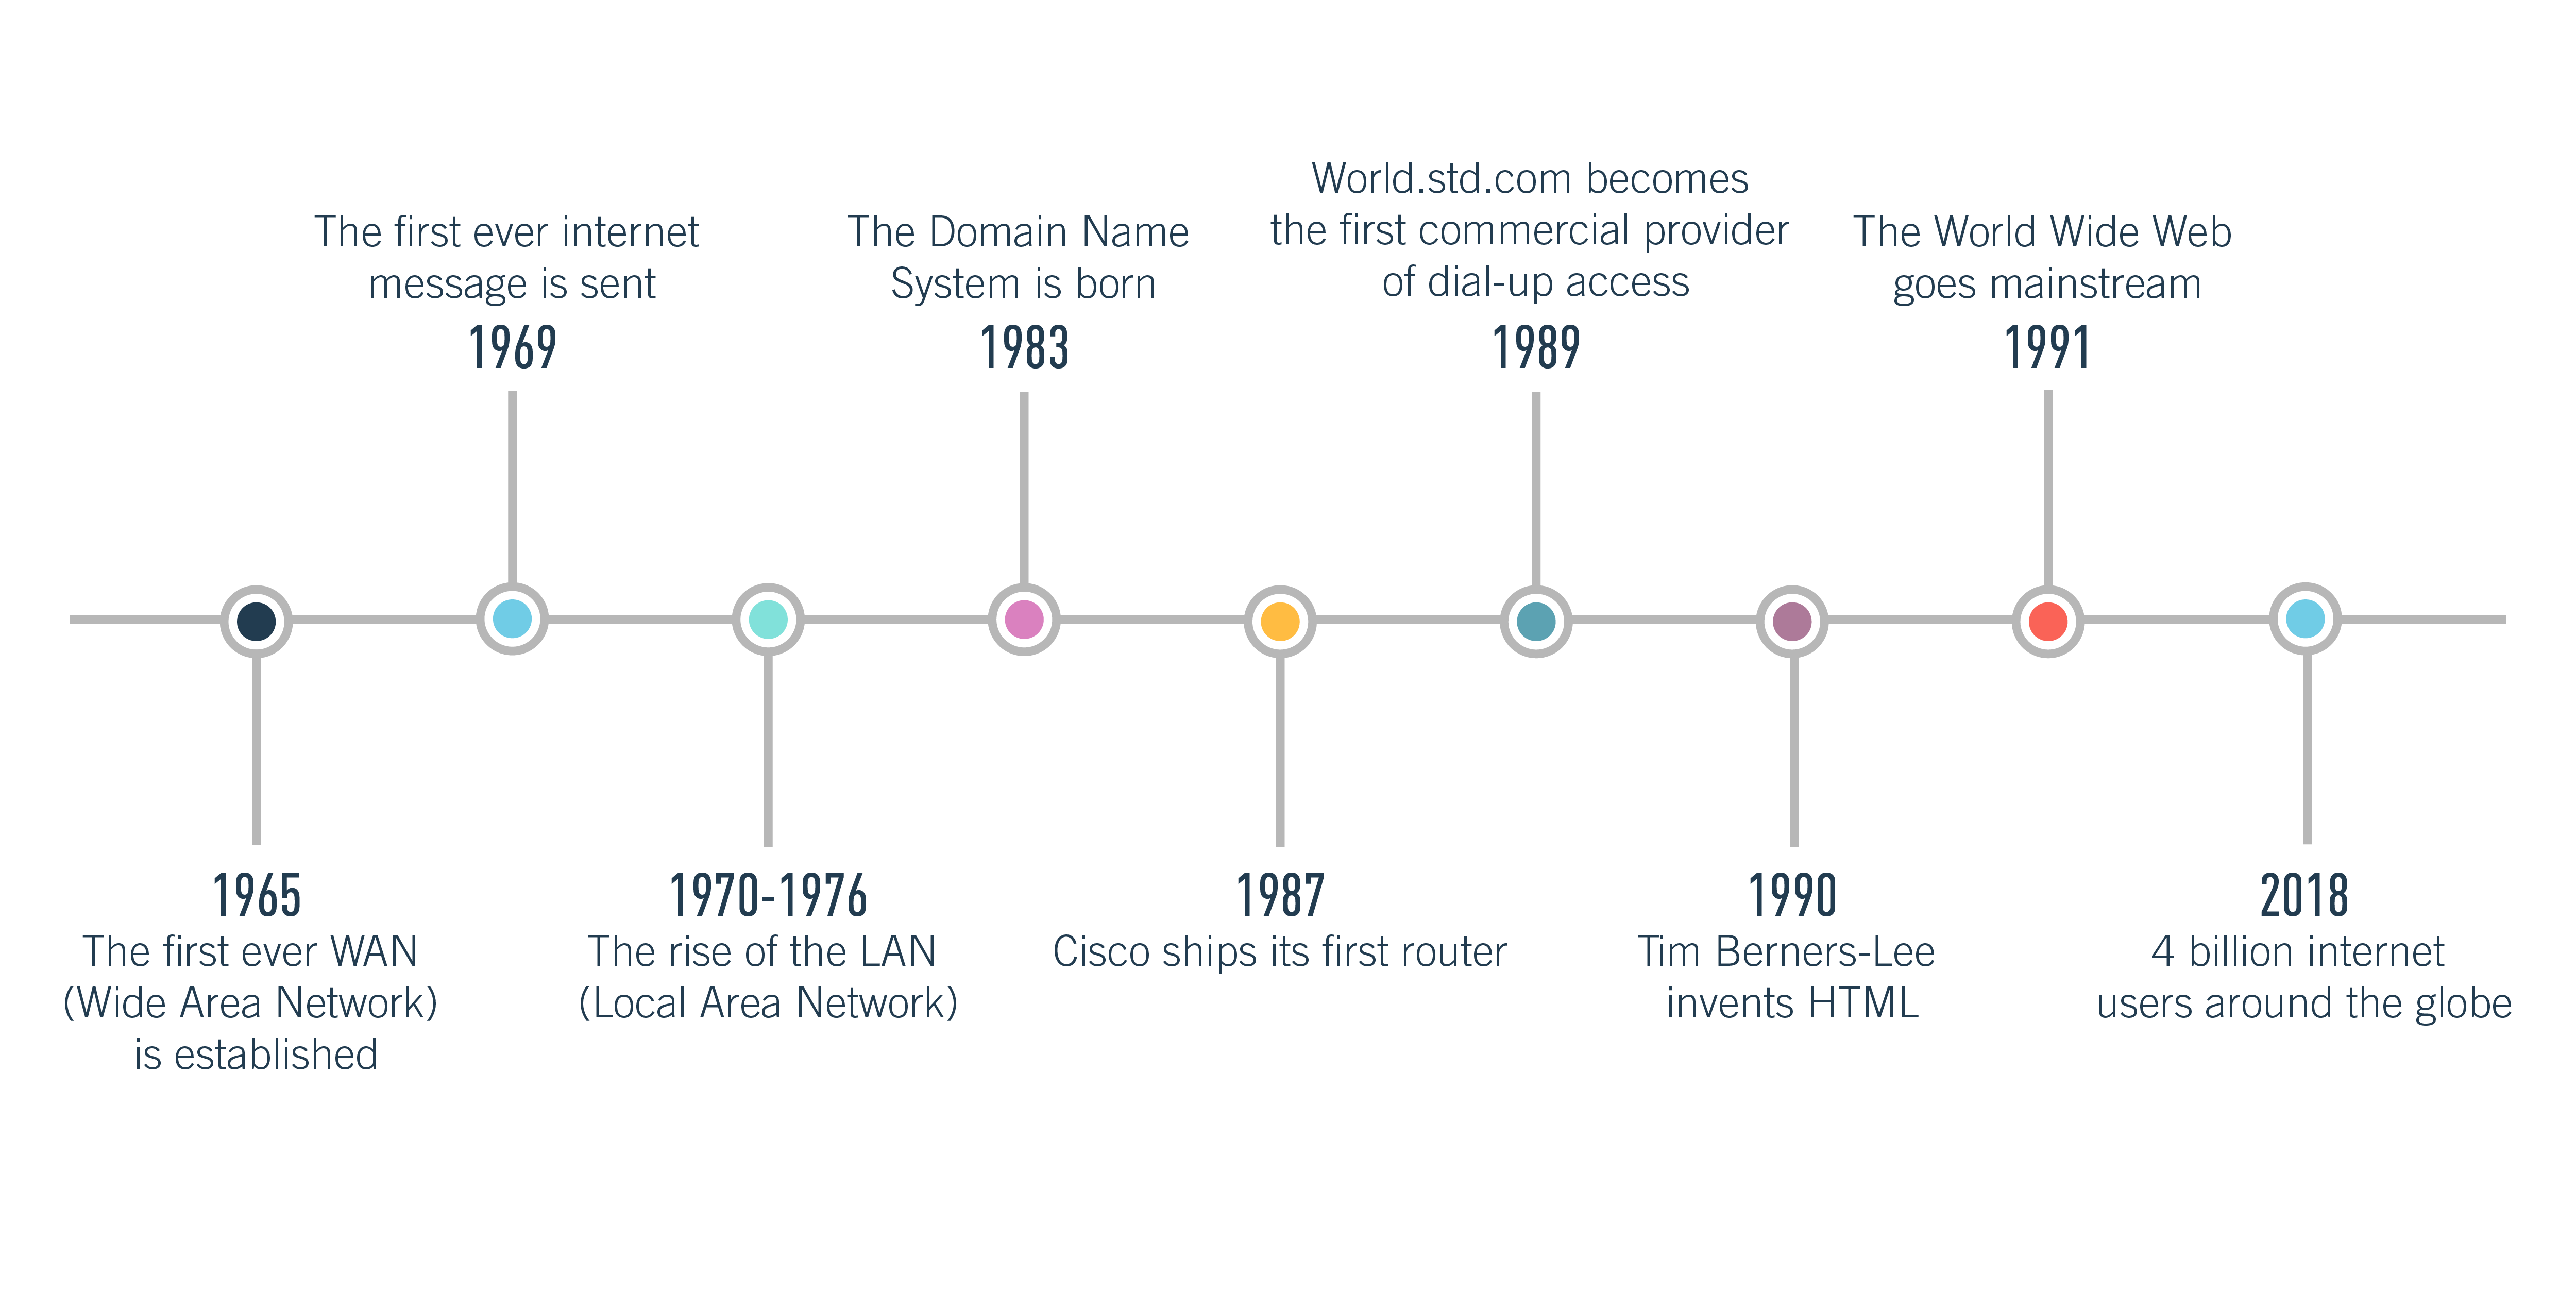
\includegraphics[width=.9\linewidth]{pictures/internet-timeline.png}
    \caption{Evolución de Internet a lo largo del tiempo, hasta llegar a hoy \cite{HowBecomeWeb}.}
    \label{fig:internet-evo}
\end{figure}

El problema a esto es evidente: con una mayor capacidad de cómputo, con más opciones
de comunicación y con más posibilidad de almacenar datos, los requisitos de las
aplicaciones van creciendo y creciendo y cada vez son más complejos de satisfacer,
no necesariamente a nivel \textit{hardware} (que por lo general suele acompañar)
sino a nivel \textit{software}. Como las aplicaciones se orientan a los usuarios
es necesario añadir capas de abstracción (como el sistema operativo) para facilitar
la labor a la persona. Sin embargo, cada capa nueva que se añade dificulta las tareas
de despliegue y mantenimiento dado que existe una gran variedad de combinaciones
\textit{hardware} y cada una puede estar con un sistema operativo distinto.

Por otra parte, la extensión de dependencias y posible incompatibilidad entre ellas
suele desembocar en el uso de versiones desactualizadas de una librería ya que tendríamos
``paquetes rotos''. Esto es tan común que tiene hasta su propio
término coloquial ``\textit{dependency hell}'' \cite{DependencyHell2021}. Contar con
dependencias obsoletas que ya han cumplido con su ciclo de vida \textit{software}
conlleva unas implicaciones de seguridad bastante severas:

\begin{itemize}
    \item Si un \textit{software} no ha mejorado a lo largo del tiempo, existe una
          malicia humana que puede aprovecharse de distintos \textit{exploits}
          existentes y comprometan nuestra aplicación.
    \item Un \textit{software} no actualizado puede tener implicaciones directas
          sobre el sistema en que se ejecuta, pudiendo producir fallos en el mismo.
          Esto se debe principalmente a que el \textit{hardware} sigue mejorando y
          creciendo y un \textit{software} antiguo puede presentar \textit{bugs}
          en dispositivos modernos que no presentaría en antiguos.
    \item Un \textit{software} no actualizado puede comprometer otros elementos del
          sistema en que se ejecuta. Por ejemplo, una aplicación `A' hace uso de dicho \textit{software}
          y una aplicación `B' también. Sin embargo, la última aplicación se ha diseñado
          para trabajar con la última versión del \textit{software} pero la aplicación
          `A' solo puede funcionar con una versión antigua e insegura. Por consiguiente,
          pese a que la aplicación `B' funcionaría correctamente el hecho de usar una
          versión antigua e insegura del \textit{software} compromete directamente al
          sistema y a la aplicación.
\end{itemize}

Es por eso que existen alternativas como ``\texttt{chroot}'' y máquinas virtuales para
subsanar estos problemas. Sin embargo, en los últimos años ha aparecido una herramienta
muy sonada y con gran éxito: Docker y los contenedores.